%%%%%%%%% Dokumentenklasse
\documentclass[
	fontsize=12pt,
	paper=a4,
	oneside,
	leqno
	]{scrartcl}


%%%%%%%%% Sprachpackages
\usepackage[T1]{fontenc}								% Textzeichen für westeuropäische Sprachen
\usepackage[utf8]{inputenc}							% Umlaute
\usepackage[ngerman]{babel}						% Automatisch erzeugte Texte werden auf Deutsch ausgegeben
\usepackage{eurosym}									% €-Symbol


%%%%%%%%% Mathe und Naturwissenschaftliche Darstellung
\usepackage[
%	fleqn															% linksbündige Formeln
	]{amsmath}												% Vielzahl von neuen Umgebungen und Befehlen für den mathematischen Bereich
\usepackage{siunitx}									% Saubere Darestellung von SI Einheiten
\sisetup{
	locale = DE,												% Deutsche Norm, Kommas werden z.B. erkannt
	per-mode=fraction,									% Output a/b as \frac{a}{b} - in der Einheit
	quotient-mode=fraction,								% Output a/b as \frac{a}{b} - im Quotienten
	fraction-function=\tfrac,
	range-phrase = {\text{~bis~}},
	sticky-per = true,										% \per bleibt bestehen für mehr als eine Einheit
	separate-uncertainty									% Standardabweichung
}
\newenvironment{conditions}						% New environment - Für saubere Darstellung gegebener Variablen
	{\par\vspace{\abovedisplayskip}\noindent\begin{tabular}{>{$}l<{$} @{${}={}$} l}}
	{\end{tabular}\par\vspace{\belowdisplayskip}}

%%%%%%%%% Schritart
\usepackage{mathptmx}								% Times New Roman


%%%%%%%%% Grafiken und Farben
\usepackage{graphicx}									% viele grafische Befehle, z.B. \scalebox
\usepackage{xcolor, colortbl}							% Farben und Farbpaletten
\usepackage[export]{adjustbox}						% Positionieren von Grafiken, left, right, center
\usepackage{float}										% Floating Bilder, H-Befehl
\usepackage{mwe} 										% Fuer Abbildungsverzeichnis
\usepackage[center]{caption} 						% Zentriert Bildunterschriften
\usepackage[labelfont={color=black,sf,it},
	font={color=black,footnotesize,it},
	labelsep=space
	]{caption}													% customise captions
\usepackage{subfigure}									%support for the manipulation and reference of small or ‘sub’ figures and tables within a single figure or table environment
\usepackage{fancybox}									% kann Boxen (Rahmen) um Elemente legen


%%%%%%%%% Seitenformatierung
\usepackage[
	headsepline,												% Vertikale Linie unterm Header
	plainheadsepline,
	automark													% Section im Header
	]{scrlayer-scrpage}									% Paket zur Manipulation der Kopf- und Fußzeilen
\renewcommand{\headfont}{}						% Voreingestellte Schriftart bearbeiten, z.B. möglich \itshape für ein feines Kursiv
\usepackage[onehalfspacing]{setspace}			% Setzt Zeilenabstand auf 1.5
\usepackage[													% optische Verbesserungen des Dokuments
	final
	]{microtype}
\usepackage[
	cache=false,												% sonst gehts nicht^^
	newfloat,													% enables you to customize the listing environment
	]{minted}													% Für Programmiersprachen
% Zu minted: unter texmaker kofigurieren pdflatex: pdflatex -synctex=1 -interaction=nonstopmode --shell-escape %.tex
% Außerdem muss python 2.7+ und pygments installiert werden. Z.B. mit anaconda
\usepackage{caption}									% Für Captions von Code

% Environment um Code mit Captions darzustellen

\newenvironment{code}{\captionsetup{type=listing}}{}
\SetupFloatingEnvironment{listing}{name=Programmcode}

%%%%%%%%% Tabellenumgebung
\usepackage{booktabs}									% enhances the quality of tables
\usepackage{array}										% extends the options for column formats
\usepackage{multirow}									% mehrzeilige Tabellenzellen
\usepackage{tabularx}									% Tabellenumgebung, praktisch für Textweite-Tabellen, Standard Column-Type: X
\newcolumntype{R}{>{\raggedleft\arraybackslash}X}	% Neuer rechtsbündiger Column-Type


%%%%%%%%% Datumsformat \today
\usepackage[ngerman, num]{isodate}				% \today im DD. MM. YYYY Format
\daymonthsepgerman{}{}								%
\monthyearsepgerman{}{}								% entfernt Leerzeichen nach den Punkten


%%%%%%%%% Kopf- und Fußzeile
\ofoot*{\today}
\cfoot{Seite \pagemark}									% Mittleres Foot-Element

%%%%%%%%% Abkürzungsverzeichnis:
%\usepackage[													% Paket für Glossaries und Acronym-Glossaries
%	acronym,
%	automake,
%	nopostdot
%	]{glossaries}

%%%%%%%%% Quellen
\usepackage[
	backend = biber,
	bibencoding = utf8,
	style = alphabetic,
	block = space,
	]{biblatex}
	

%%%%%%%%% Formatierung TOC
\usepackage{tocstyle}
\newtocstyle[KOMAlike][leaders]{alldotted}{}	% Punktlinienführung, wie Abbildungs- und Tabellenverzeichnis
\usetocstyle{alldotted}

	
%\usepackage{tocloft}
%\setlength\cftparskip{0pt}
%\setlength\cftbeforesecskip{0pt}
%\setlength\cftaftertoctitleskip{1pt}

\usepackage[													% Zum Schluss laden, wegen Komplikationen
	hidelinks													% keine Boxen um die Links im PDF
	]{hyperref}												% Zulassen von Links u.ä. im PDF File																		% Präambel

% Shortcuts for SI Values
% Grundlagen: https://www.namsu.de/Extra/pakete/Siunitx.html
% Gute Erklärung der Shortcuts: https://texwelt.de/fragen/2588/wie-schreibe-ich-zahlen-mit-einheiten-richtig

%\DeclareSIUnit{\BeladungsDichte}{\kilo\gram_{\textup{H\textup{2}}\per\kilo\gram_{\textup{FeTi}}}}		% Beladungsdichte
%\DeclareDocumentCommand\BeladungsDichte{O{}m}{\SI[#1]{#2}{\BeladungsDichte}}

%\DeclareSIUnit[]\NormVolumen
%{\text{\ensuremath{\cubic\meter_{\textup{i.N.}}}}}

%%%%%%% New SIValues

\DeclareSIUnit{\sieuro}{\mbox{\euro}}
\DeclareSIUnit\ct{ct}
\DeclareSIUnit\kgh{\kg_{H\textsubscript{2}}}
\DeclareSIUnit\kgfe{\kg_{FeTi}}
\DeclareSIUnit\normvol{\cubic\meter_{i.N.}}
\DeclareSIUnit\normvolL{\liter_{i.N.}}
\DeclareSIUnit\kw{\kilo\watt}
\DeclareSIUnit\kwh{\kilo\watt\hour}
\DeclareSIUnit\kwp{\kilo\watt_{p}}
\DeclareSIUnit\ctkwh{\ct\per\kwh}
\DeclareSIUnit\Eurkwh{\sieuro\per\kwh}

%%%%%%% New complete Commands

\NewDocumentCommand\DeclareNewQuantity{mmm}{%
	\DeclareSIUnit{#2}{#3}%
	\DeclareDocumentCommand{#1}{O{}m}{\SI[##1]{##2}{#2}}%
}

\DeclareNewQuantity
	\Beladungsdichte
	\beladungsdichte
	{\kgh\per\kgfe}
\DeclareNewQuantity
	\Dichte
	\dichte
	{\kg\per\cubic\meter}
\DeclareNewQuantity
	\Faraday
	\faraday
	{\ampere\second\per\mol}
\DeclareNewQuantity
	\Molarvolumen
	\molarvolumen
	{\liter\per\mol}
\DeclareNewQuantity
	\Normvolumen
	\normvolumen
	{\normvol}
\DeclareNewQuantity
	\Normvolumenstrom
	\normvolumenstrom
	{\normvolL\per\minute}
\DeclareNewQuantity
	\Normvolumenstromsec
	\normvolumenstromsec
	{\normvolL\per\second}
\DeclareNewQuantity
	\Volumenstrom
	\volumenstrom
	{\liter\per\minute}																			% Abkürzungen für lange SI-Einheiten-Kombinationen

\addbibresource{Sources.bib}															% Quellen-Datein Pfad angeben

\begin{document}

\begin{titlepage}
	\begin{center}
	
		\thisfancyput(3.125in,-4.5in){%
			\setlength{\unitlength}{2.5cm}\fancyoval(7,9.5)}
		
		\vspace*{1cm}
		
		\textbf{\textsc{{\huge Dokumentation}}}
 
		\vspace{0.5cm}

		{\Large Primärregelleistungserbringung\\\medskip\noindent eines dezentralen virtuelles Kraftwerk}
 
		\vspace{0.5cm}

		Berlin, \today
       
		\vspace*{1cm}
       
		\begin{figure}[H]
			
\includegraphics[width=0.5\textwidth, center]{Bilder/HTWLogo.jpg}
		\end{figure}
 
		\vfill
 
		\vspace{0.8cm}
 
		\begin{minipage}{0.4\textwidth}
			\begin{flushleft}
				\textbf{Studiengang:}\\
				\textbf{Fachbereich:}\newline\newline
				\textbf{Gruppe:}\\
				\textbf{Autoren:}\newline\newline
				\textbf{Prüfer:}\\
			\end{flushleft}
		\end{minipage}~
		\begin{minipage}{0.4\textwidth}            
			\begin{flushright}
				Regenerative Energien (M)\\
				Ingenieurwissenschaften – Energie und Information\\
				N\\
				Kilian Helfenbein\\
				Michaela Zoll\\
				Johannes Weniger\\
			\end{flushright}        
		\end{minipage}\\[2 cm]
		
	\end{center}
\end{titlepage}

\newpage																			% Titelblatt

% ToC, Abbildungsverzeichnis, Tabellenverzeichnis und Akronyme

\pagenumbering{Roman}																	% Roman Page Numbers

\begin{spacing}{1}																			% Spacing auf 1 statt 1.5 setzen, damit ToC O.K. aussieht
	\tableofcontents																				% Inhaltsverzeichnis
\end{spacing}

\newpage

\addcontentsline{toc}{section}{Abbildungsverzeichnis}						% Abbildungsverzeichnins
\begin{spacing}{1}
	\listoffigures
\end{spacing}

%\newpage

%\addcontentsline{toc}{section}{Tabellenverzeichnis}							% Tabellenverzeichnis
%\begin{spacing}{1}
%	\listoftables
%\end{spacing}

%\newpage

%\addcontentsline{toc}{section}{Akronyme}									% Abkürzungsverzeichnis erzeugen
%\begin{spacing}{1}
%	\printglossary[type=\acronymtype]
%\end{spacing}

\newpage

\pagenumbering{arabic}																	% Arabic Page Numbers


% Vorbereitungsfragen

\section{Vorbereitungsfragen}

																				% Einleitung

% Theoretische Grundlage, Berechnungsmethodik und Datensätze

\section{Theoretische Grundlagen und Datengrundlage}

In diesem Kapitel sollen die wichtigsten Grundlagen erläutert werden, um eine Bewertung des Einflusses der Nutzung des Speichersystems für die Erbringung von Primärregelleistung vornehmen zu können. Hierzu zählen die theoretischen Grundlagen der Erbringung von Primärregelleistung und des virtuellen Kraftwerks inklusive der verwendeten Hardware. Weiterhin wird auf die wichtigsten verwendeten Python und Matlab Befehle, sowie die verwendeten Datensätze und deren Aufarbeitung eingegangen. Zusätzlich wird das Vertragsmodell der sonnenFlat erläutert, um die Kostenstruktur darstellen zu können.

\subsection{Primärregelleistung}

Um zukünftig die Versorgungssicherheit gewährleisten zu können, müssen nicht nur erhebliche Mengen an Kraftwerksleistungen regenerativer Energieanlagen zugebaut werden, sondern auch die Erbringung von Systemdienstleistungen garantiert werden, welche bisher zum großen Teil durch konventionelle Großkraftwerke gedeckt werden. Ein wichtiger Baustein ist die Aufrechterhaltung der Netzfrequenz, welches durch die Erbringung von Regelleistung ermöglicht wird. Diese Simulation soll sich mit der Erbringung von Primärregelleistung befassen, welches die schnellste Art der Regelleistung im europäische Verbundsystem darstellt.\medskip\\
Der Zweck der Primärregelleistung liegt darin, die Netzfrequenz durch gezielte Leistungserbringung zu stabilisieren. Nötig wird dies, wenn eine Differenz zwischen dem Angebot und der Nachfrage an Leistung im Stromnetz besteht. Die Leistungserbringung wird automatisch durch eine Frequenzabweichung von der Soll-Netzfrequenz von \SI{50}{\hertz} aktiviert. Dabei wird durch die Übertragungsnetzbetreiber ein Totband von $\pm \SI{10}{\milli\hertz}$ definiert, in welchem keine Erbringung von Primärregelleistung erfolgen muss. Bei einer Abweichung von $\pm \SI{200}{\milli\hertz}$ muss hingegen die volle ausgeschriebene Regelleistung des Kraftwerks erbracht werden und dazwischen proportional zu der Frequenzabweichung \parencite{nextKW20}.


\subsection{sonnenBatterie eco 8.0}\label{sec:SB_eco8_Theorie}

Ein Schwarm aus Heimspeichern der sonnenBatterie eco 8.0 Serie bildet die physische Grundlage des virtuellen Kraftwerks. Bei der eco 8.0 handelt es sich um einen Lithium-Eisenphosphat-Akkumulator, dessen wesentlichen technischen Eigenschaften die Möglichkeiten des gesamten virtuellen Kraftwerks begrenzen.\\
Die einzelnen Batterien besitzen je nach Ausstattung eine nutzbare Batteriekapazität von \SIrange{4}{16}{\kwh}. Vereinfachend wird angenommen, dass nur sonnenBatterien mit einer Kapazität von mindestens \SI{8}{\kwh} eingesetzt werden. Ab einer Kapazität von  \SI{8}{\kwh} ist jede Batterie  mit einem Wechselrichter ausgestattet, der eine Nennleistung von \SI{3.3}{\kilo\watt} besitzt \parencite{sonnenBat18}.\\
Der mittlere Wirkungsgrad des Wechselrichters beträgt im Entladefall \SI{94.5}{\percent} und im Ladefall \SI{94.4}{\percent}. Weiterhin weißt die Batterie einen Wirkungsgrad von \SI{93.8}{\percent} auf \parencite{htwInspek19}.

\subsection{Das virtuelle Kraftwerk}\label{sec:VK_Theorie}

Das virtuelle Kraftwerk der Simulation wurde mit einer Gesamtleistung von \SI{1}{\mega\watt} präqualifiziert. Als Annahme wurden hierzu insgesamt 600 Heimspeicher der sonnenBatterie eco 8.0 Serie vernetzt, mit einer Gesamtleitung von \SI{1.98}{\mega\watt}. Der theoretische Leistungsspielraum des Kraftwerks liegt somit deutlich über der präqualifizierten Leistung.\\
Nötig ist dies aus verschiedenen Gründen. So kann beispielsweise nicht die Verfügbarkeit jeder Batterie zu jedem Zeitpunkt garantiert werden. Die einzelnen Batterien befinden sich in Privathand und unterliegen somit nur begrenzt der Kontrolle durch den Betreiber. Es kann zu Störungen der Hard- oder Software der einzelnen Batterien kommen, aber auch zu Störungen der Internetverbindung.\\
Die größten beschränkenden Faktoren des virtuellen Kraftwerks sind jedoch der Ladestand und der aktuelle Arbeitspunkt. Der Arbeitspunkt bestimmt, wie viel Regelleistung in positiver bzw. negativer Regelrichtung zur Verfügung steht. Als Regelleistung wird die Abweichung vom Arbeitspunkt verstanden. Der Arbeitspunkt der Batterien entspricht der eigenverbrauchsoptimierten Leistungsvorgabe.\\
Wenn der Ladestand zu gering bzw. zu hoch ist, kann die Erbringung der Regelleistung nicht in der gewünschten Dauer erfolgen. Bei einem zu hohen bzw. zu niedrigen Arbeitspunkt des Batteriepools kann das Kraftwerk bei einem Leistungsabruf nicht die geforderte Regelleistung erbringen. Durch aktives Lademanagement und das Einhalten von Grenzen für den Ladezustand muss im Realbetrieb die Erbringung der präqualifizierten Regelleistung garantiert werden.\\
Das grundlegende Funktionsprinzip des virtuellen Kraftwerks wird durch einen übergeordneten Regler bestimmt. Dieser wird in der Simulation stark vereinfacht. So wird von einem homogenen Verhalten der Batterien ausgegangen. Dies bedeutet, dass jede Batterie  die gleichen technischen Parameter besitzt und das sich die zugehörigen Photovoltaikanlagen ebenfalls identisch verhalten. Das führt dazu, dass den einzelnen Batterien feste Ladestandsgrenzen zugeordnet werden können, damit die Erbringung von Regelleitung im Bedarfsfall gewährleistet werden kann.

\begin{figure}[H]
	\begin{center}
		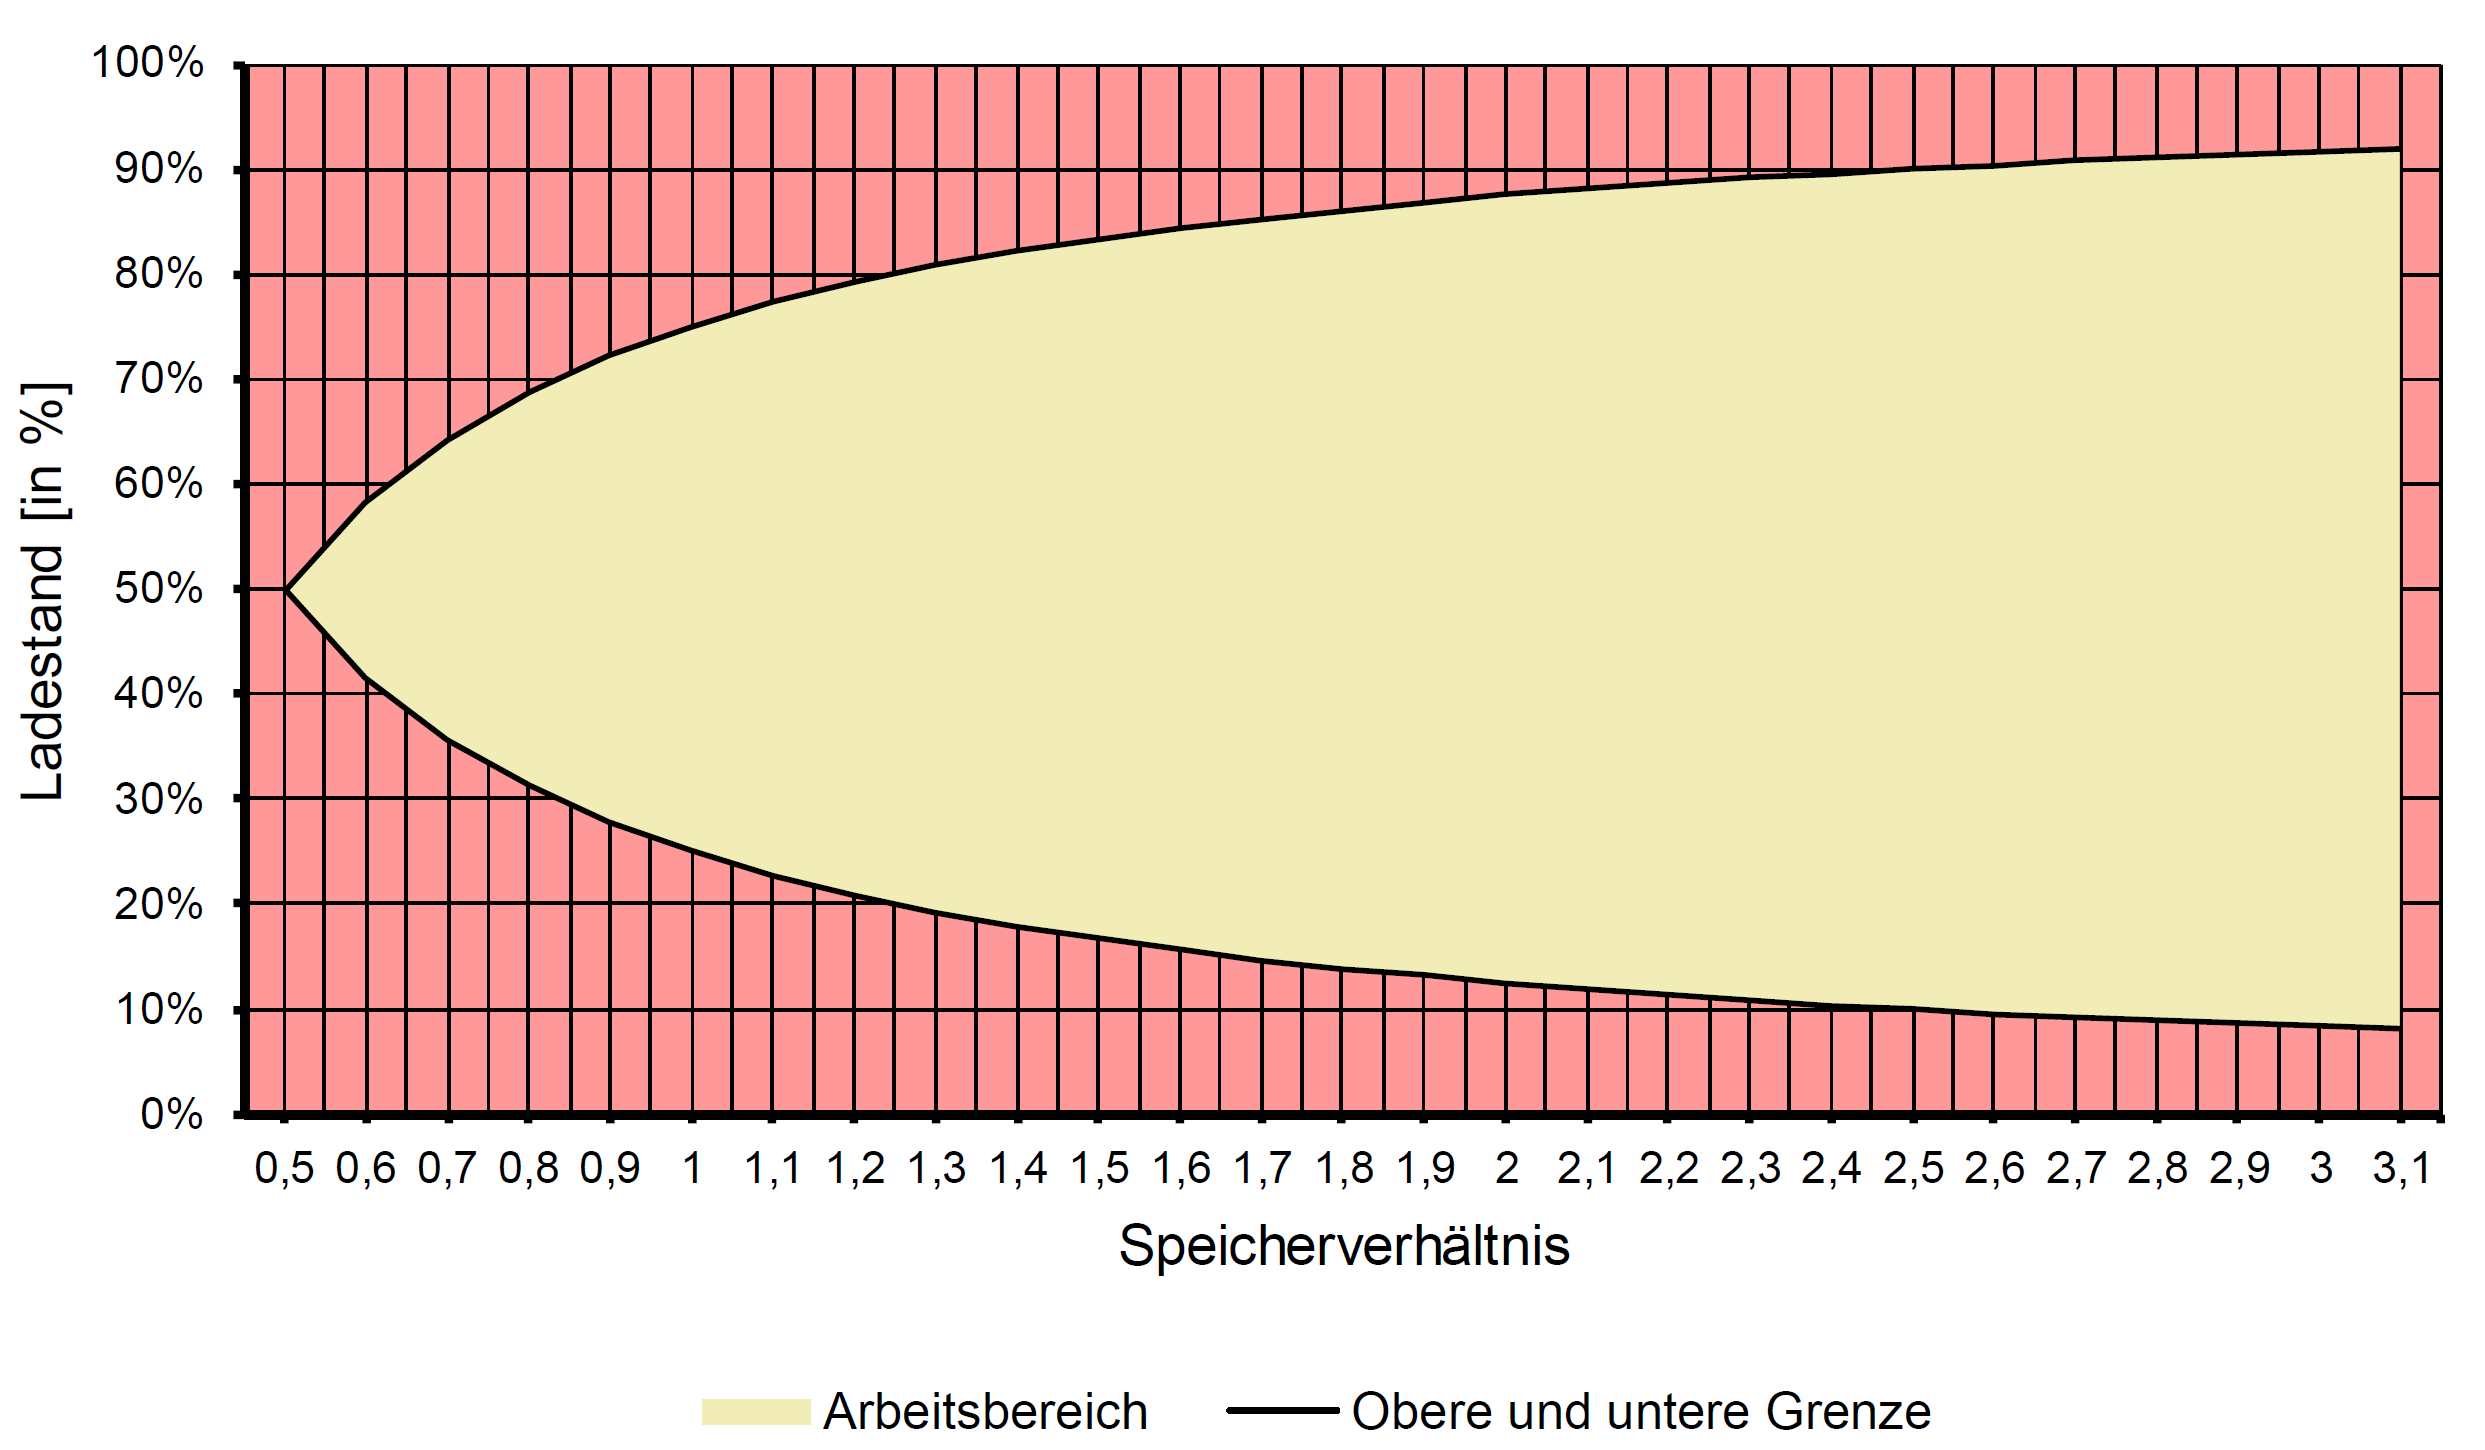
\includegraphics[width=\textwidth]{Bilder/P-E_factor.png}
		\caption{Zulässiger Arbeitsbereich bei der Erbringung von Primärregelleistung \parencite[s. S. 61][]{regel_PQ19}}
		\label{fig:P_E_factor}
	\end{center}
\end{figure}

\noindent Im Falle begrenzter Energiespeicher kommen die in Abbildung \ref{fig:P_E_factor} dargestellten zulässigen Arbeitsbereiche zur Anwendung. Durch dies wird sichergestellt, dass der Energiespeicher jederzeit seine vollständige angebotene Regelleistung für \SI{15}{\minute} zur Verfügung zu stellen.\medskip\\
In dem Fall des simulierten virtuellen Kraftwerks besteht ein Speicherverhältnis von \SIrange{4.8}{9.6}{}, je nach Größe der einzelnen Speichereinheiten. Da jedoch das Lademanagement innerhalb dieser Simulation nicht abgebildet werden kann, wurde sich für Ladestandsgrenzen von \SI{80}{\percent} im oberen und \SI{20}{\percent} im unteren Energiebereich entschieden.

\subsection{Die sonnenFlat}

Das Konzept der sonnenFlat beruht in erster Linie auf der sogenannten Freistrommenge. Diese dient als Leistungstausch für die Einschränkungen des eigenverbrauchsoptimierten Verhaltens der Batterie. Die Freistrommenge bezieht sich auf den Gesamtstromverbrauch und beinhaltet den Direktverbrauch der Photovoltaikanlage und den zusätzlichen Netzbezug. Der Netzbezug der Batterie für die Erbringung von Primärregelleistung wird getrennt bilanziert.

\begin{figure}[H]
	\begin{center}
		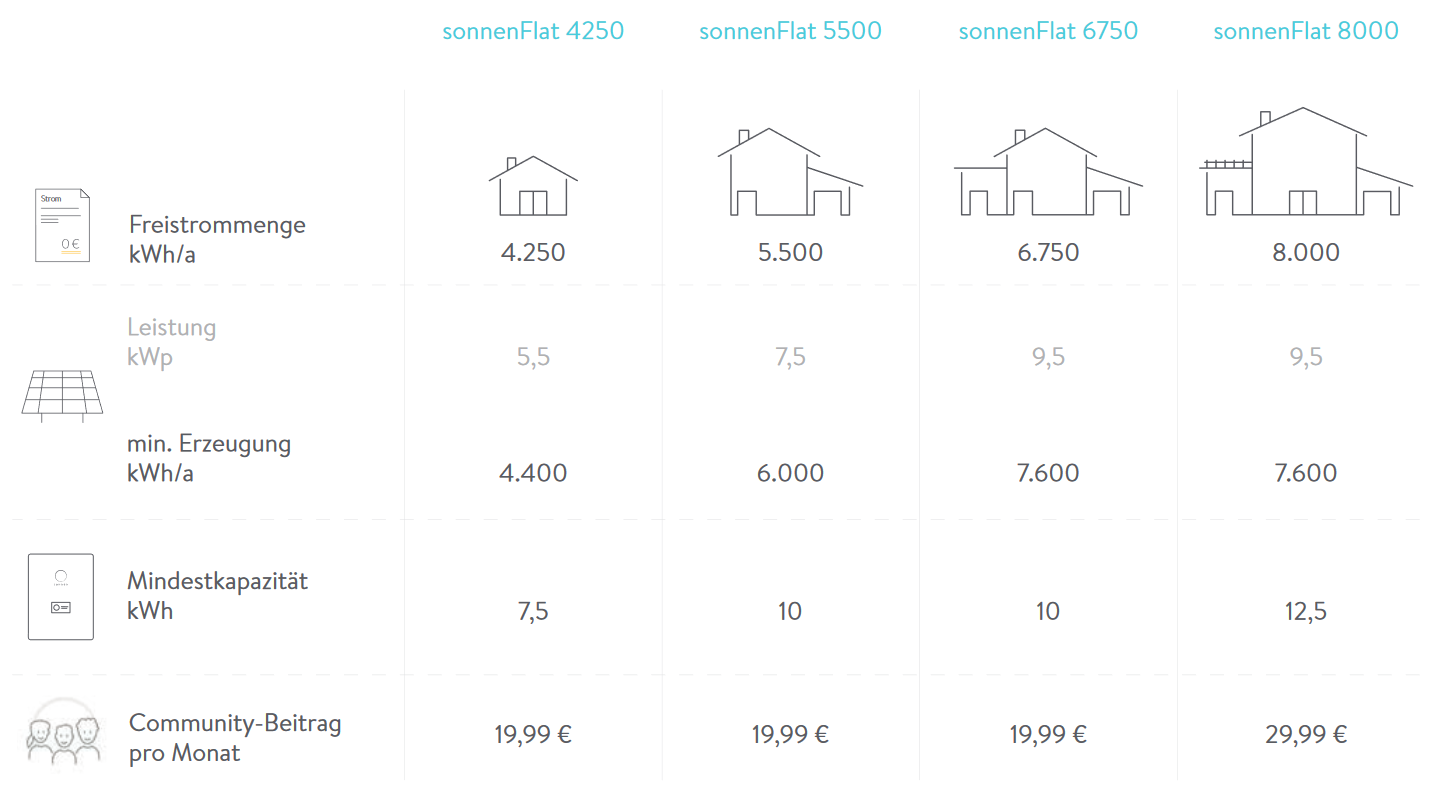
\includegraphics[width=\textwidth]{Bilder/flat.png}
		\caption{Varianten der sonnenFlat \parencite[s. S. 26][]{flat20}}
		\label{fig:flat_ver}
	\end{center}
\end{figure}

\noindent In Abbildung \ref{fig:flat_ver} sind die verschiedenen Varianten der sonnenFlat vorgegeben. Die Freistrommenge des Kunden hängt sowohl von der Leistung der Photovoltaikanlage und der Kapazität des Batteriespeichers ab. Die minimale Größe der Photovoltaikanlage beträgt hierbei \SI{5.5}{\kwp}, weshalb dies als minimale Größe der Simulation angenommen wurde. In dieser Simulation wird davon ausgegangen, dass der Kunde immer die für seine spezielle Situation größtmögliche sonnenFlat erhält. Hiervon ausgenommen ist die sonnenFlat 8000, da bei dieser höhere Community-Beiträge anfallen. Bei Überziehung der Freistrommenge von bis zu \SI{2000}{\kwh}, fallen bei der sonnenFlat Arbeitspreise von \SI{23}{\ctkwh} und darüber \SI{25.9}{\ctkwh} an \parencite{flat20}. Der Break-even-Point der sonnenFlat 8000 gegenüber der sonnenFlat 6750 ist somit ab einem jährlichen Stromverbrauch von \SI{7272}{\kwh} erreicht.\medskip\\
Eine weitere Besonderheit des sonnenFlat Vertrages ist der sogenannte sonnenBonus.. Hierbei handelt es sich um einen Aufschlag von  \SI{0.25}{\ctkwh} für jede eingespeiste Kilowattstunde der Photovoltaikanlage auf die übliche EEG-Vergütung \parencite{sonnenBonus20}.

\subsection{Verwendete Python und Matlab Befehle}

In diesem Kapitel werden die wichtigsten Python und Matlab Befehle erklärt. Auf Befehle, die bereits Teil der Vorlesung waren, wird nicht eingegangen.

\subsubsection*{Python}

\textbf{Glob}\\
Das \texttt{Glob}-Modul findet alle Pfadnamen, die mit einem angegebenen Muster übereinstimmen \parencite{PyGlob20}.\medskip\\

\noindent\textbf{Pandas}\\
\texttt{Pandas} bietet Funktionen für die Strukturierung und Analyse von Datensätzen \parencite{PyPan20}. Die wichtigsten verwendeten Befehle der \texttt{Pandas}-Bibliothek lauten wie folgt:

\begin{conditions}
	\text{\texttt{read\_csv()}}		&		Einlesen einer CSV-Datei als Datenfeld\\
	\text{\texttt{DataFrame()}}	&		Erstellt ein Datenfeld mit gewünschten Parametern\\
	\text{\texttt{multiply()}}		&		Ermöglicht Multiplikation eines Datenfeldes mit einem Skalar\\
	\text{\texttt{round()}}			&		Runden der Elemente eines Datenfeldes\\
	\text{\texttt{to\_csv()}}			&		Speichern eines Datenfeldes als CSV-Datei\\
	\text{\texttt{concat()}}			&		Verketten von einzelnen Datenfeldern\\
\end{conditions}


\subsubsection*{Matlab}

\textbf{Polyval}\\
Der Befehl \texttt{polyval(p, x)} wertet ein Polynom \texttt{p} an jedem Punkt in \texttt{x} aus. Das Argument \texttt{p} ist ein Vektor der Länge \texttt{n $+$ 1}, dessen Elemente die Koeffizienten (in absteigenden Potenzen) eines Polynoms \texttt{n}-ten Grades sind \parencite{MatPol20}:

\[ p\left(x\right)	= p_1 \cdot x^n + p_2 \cdot x^{n-1} + ... + p_n \cdot x + p_{n+1}	\]

\noindent\textbf{Reshape}\\
\texttt{Reshape} formt ein gegebenes Array in eine gewünschte Form um. Beispielsweise formt \texttt{reshape(A, [2,3])} \texttt{A} in eine 2-mal-3-Matrix um \parencite{MatRe20}.

\subsection{Datengrundlage}

Für die Simulation des Einflusses des virtuellen Kraftwerks kamen drei Datensätze zum Einsatz. Hierzu zählt ein Haushaltslastprofil, das Erzeugungsprofil einer Photovoltaikanlage und das Profil der Netzfrequenz im europäische Verbundsystem, welche modellexogen die Grundlage der Simulation bilden. Jeder Datensatz hat eine 1-minütige Auflösung und bildet ein ganzes Jahr ab. Die Aufarbeitung der einzelnen Datensätze erfolgt mit Hilfe von Python.

\subsubsection{Erzeugungsprofil der Photovoltaikanlage}

Das Erzeugungsprofil der Photvoltaikanlage wurde innerhalb der Vorlesung zur Verfügung gestellt. Dieses findet auch hier Anwendung und ist in der Datei \texttt{A04\_Daten.mat} hinterlegt. In der Variable \texttt{ppvs} ist die spezifische AC-Leistungsabgabe des Photovoltaik-Systems, normiert auf die nominale Photovoltaik-Generatorleistung hinterlegt.

\subsubsection{Haushaltslastprofil}

Das Haushaltslastprofil entspricht einem repräsentativen elektrische Lastprofile für Wohngebäude in Deutschland auf 1-minütiger Datenbasis. Dieses wird durch die Hochschule für Technik und Wirtschaft Berlin zur Verfügung gestellt \parencite{htwLast18}.\\
Verwendet wurde das dritte Lastprofil der Datei \texttt{CSV\_74\_Loadprofiles\_1min\_W\_var(1).zip}. Auch dieses wurde normiert. Dafür wurde zuvor die maximale Leistungaufnahme des Systems bestimmt und mit dieser die spezifische Leistungsaufnahme des Systems zu jeder Minute ermittelt.\medskip\\
Realisiert wurde dies mit folgendem Code:

\begin{code}
\captionof{listing}{Aufbereitung des Datensatzes des repräsentativen elektrischen Lastprofils für Wohngebäude}
\label{code:household}
\begin{minted}{python}
import pandas as pd

# Namen für die Spalten des Datensatzes bestimmen
names = list()
for i in range(74):
    names.append('H{}' .format(i+1))
    
# Einlesen der Daten
df_Load1 = pd.read_csv('DataRaw\\PL1.csv', names=names, sep=',')

# Ziel Datensatz isolieren und normieren
df_Household = pd.DataFrame()
df_Household['P_H'] = df_Load1.H3.multiply(1/max(df_Load1.H3))

# Speichern als .csv und runden
df_Household.round(5).to_csv('P_H.csv')
\end{minted}
\end{code}

\subsubsection{Profil der Netzfrequenz}

Das Profil der Netzfrequenz im europäische Verbundsystem liegt in 1-sekündiger Auflösung monatsweise für das Jahr 2018 vor. Zur Verfügung gestellt wurden die entsprechenden Datensätze durch Herrn Dipl.-Ing. (FH) Markus Jaschinsky \parencite{Jaschinsky18}.\medskip\\
Ziel der Aufarbeitung war es die einzelnen Profile zusammenzuführen und in eine 1-minütige Auflösung umzuwandeln. Anschließend sollte aus diesem Profil der Lastgang des virtuellen Kraftwerks, normiert auf die ausgeschriebene Primärregelleistung, ermittelt werden. Dieses erfolgte auf Grundlage des folgenden Codes:

\begin{code}
\captionof{listing}{Aufbereitung der Datensätze des Profils der Netzfrequenz im europäische Verbundsystem}
\label{code:VPP}
\begin{minted}{python}
import glob
import pandas as pd

# Namen der einzelnen Datein ermitteln
lst_csv = glob.glob("2018\*.csv", recursive=True)
# Spaltennamen festlegen
names = ['fq', 'delete']

# Ergebnisliste vorinitialisieren
lst_df = [0]*len(lst_csv)
i = 0

# Einlesen der einzelnen Datensätze
for name in lst_csv:
    lst_df[i] = pd.read_csv(name, names=names, sep=';')
    lst_df[i].index.name = 'ts'
    lst_df[i] = lst_df[i].drop(['delete'], axis=1)
    i += 1
    
# Zusammenführen der Monatsdatensätze
df_fq18 = pd.DataFrame()

for n in range(len(lst_df)):
    df_fq18 = pd.concat([df_fq18, lst_df[n]], sort=False)
    
# Umwandeln in 1-minütige Auflösung
df_fq18_minutes = df_fq18.copy().iloc[::60, :]

# Umrechnen der Netzfrequenz
# in die Sollvorgabe der Leistungserbringung des VPP
df_fq18_minutes['p_VPP'] =
[0 if 49.99 < fq < 50.01 else (50 - fq)*10/2 for fq in df_fq18_minutes.fq]

# Speichern als .xlsx
df_fq18_minutes.round(3).to_excel('P_VPP.xlsx')
\end{minted}
\end{code}

\newpage																			% Theorie

% Hauptteil

\section{Simulation des Batteriespeichersystems}

In diesem Kapitel werden die wichtigsten Simulationsschritte dargestellt und erläutert. Weiterhin erfolgt eine Betrachtung der Ergebnisse.

\subsection{Parametervariation und Simulationsziele}

Die Parametervariation soll dazu dienen, möglichst viele Fälle möglichst genau darstellen zu können. Folgende Parameter fließen modellendogen in die Durchläufe der Simulation ein:

\begin{itemize}
\itemsep-0.5em
	\item Der Hausverbrauch von \SIrange{3000}{10000}{\kwh}
	\item Die Kapazität der Batterie von \SIrange{8}{16}{\kwh}
	\item Die Größe der Photovoltaikanlage von \SIrange{5.5}{10}{\kwp}
	\item Die EEG-Vergütung für die Stromeinspeisung von \SIrange{9.87}{12.75}{\ctkwh}
	\item Der Grundpreis des Vergleichstromtarifs von \SIrange{5}{12}{\Eurkwh}
	\item Der Arbeitspreis des Vergleichstromtarifs von \SIrange{25}{32}{\ctkwh}
\end{itemize}

\noindent Weiterhin sind folgende Parameter modellexogen vorgegeben und nicht variiert:

\begin{itemize}
\itemsep-0.5em
	\item Die nominale AC-Leistungsaufnahme des Batteriewechselrichters \SI{3.3}{\kw}
	\item Die nominale AC-Leistungsabgabe des Batteriewechselrichters \SI{3.3}{\kw}
	\item Der mittlerer Umwandlungswirkungsgrad des Batteriewechselrichters im Ladebetrieb \SI{94.4}{\percent}
	\item Der mittlerer Umwandlungswirkungsgrad des Batteriewechselrichters im Entladebetrieb \SI{94.5}{\percent}
	\item Der mittlerer Umwandlungswirkungsgrad des Batteriespeichers \SI{93.8}{\percent}
	\item Die präqualifizierte Leistung des virtuellen Kraftwerks $\pm \SI{1}{\mega\watt}$
	\item Die theoretische maximale Leistung des virtuellen Kraftwerks $\pm \SI{1.98}{\mega\watt}$
	\item Der sonnenBonus in Höhe von \SI{0.25}{\ctkwh}
\end{itemize}

\noindent Das Ziel der Simulation ist es, in erster Linie einen Kostenvergleich der Vertragsvarianten für den Kunden zu ermöglichen. Die wichtigsten zu ermittelten Größen sind von daher die jährlichen Kosten. Außerdem soll ermittelt werden, wie stark die Batterie durch das virtuelle Kraftwerk mehr belastet wird. Hierfür werden die auftretenden Vollzyklen pro Jahr berechnet.

\subsection{Simulation des Einflusses des virtuellen Kraftwerks}

Dieses Kapitel soll die Simulation des Einflusses des virtuellen Kraftwerks auf das eigenverbrauchsoptimierte Verhalten der Batterie erläutern. Weiterhin soll eine Bewertung der Approximation vorgenommen werden.

\subsubsection{Erläuterung der Simulation}

Die Erbringung von Primärregelleistung hat immer Vorrang vor der Eigenverbrauchsoptimierung des Kunden. Somit muss ermittelt werden, in welchen Zeitschritten es zu einer Erbringung von Primärregelleistung kommt.\medskip\\
Als erste Approximation wird angenommen, dass das virtuelle Kraftwerk an \SI{80}{\percent} der Tage des Jahres an der Erbringung von Primärregelleistung teilnimmt. Hierdurch werden Wartung und nicht erfolgreiche Ausschreibungen abgedeckt. Um einen ausreichenden Ladestand zu garantieren, wird weiterhin zwischen zwei Zuständen unterschieden:

\begin{enumerate}
\itemsep-0.5em
	\item Die Ladestandsgrenzen sind aktiviert
	\item Die Erbringung von Primärregelleistung und die Ladestandsgrenzen sind aktiviert
\end{enumerate}

\noindent Der erste Fall tritt immer dann auf, wenn auf einen Tag ohne Erbringung von Primärregelleistung ein regelleistungsaktiver Tag folgt. In diesem Fall werden die Ladestandsgrenzen von \SIrange{20}{80}{\percent} bereits \SI{12}{\hour} vor der eigentlichen Erbringung aktiviert. Damit soll möglichst sichergestellt werden, dass zu Beginn der Regelleistungserbringung genügend Energie in den Speichern zur Verfügung steht. Weiterhin soll auf diese Weise auf eine Simulation des Nachlademanagements des virtuellen Kraftwerks verzichtet werden können.\medskip\\
Im nächsten Schritt, muss ermittelt werden ob die eigene Batterie in dem vorliegenden Zeitschritt an der Erbringung von Primärregelleistung teilnimmt. Hierfür wurde ein einfacher boolean Minuten-Vektor geschaffen, mit folgenden Bedeutungen:

\begin{itemize}
\itemsep-0.5em
	\item $0 =$ Eigenverbrauchsoptimierung
	\item $1 =$ Erbringung von Primärregelleistung
\end{itemize}

\noindent Damit die Batterie an der Regelleistungserbringung teilnimmt, muss die Regelleistungserbringung des gesamten virtuellen Kraftwerks aktiv sein, die Frequenzabweichung der Netzfrequenz außerhalb des Totbandes liegen und die Batterie zu den verwendeten Batterien des Zeitschritts gehören.\\
Um die letzte Vorraussetzung zu approximieren, wurde vorerst die Wahrscheinlichkeit berechnet, dass die Batterie Primärregelleistung in dem Zeitschritt erbringen muss.

\begin{equation}
\label{eq:approx_FCR}
	p_{\text{FCR}}\left(t\right) = \left|P_{\text{FCR}_{\text{VPP}}}\left(t\right)\right| \cdot \frac{P_{\text{PQ}}}{P_{\text{max}}}
\end{equation}

\begin{conditions}
	t															&		Zeitschritt\\
	p_{\text{FCR}}\left(t\right)					&		Wahrscheinlichkeit der Regelleistungserbringung\\
	P_{\text{FCR}_{\text{VPP}}}\left(t\right)	&		Abgerufene Primärregelleistung des virtuellen Kraftwerks im Zeitschritt\\
	P_{\text{PQ}}										&		Präqualifizierte Leistung des virtuellen Kraftwerks\\   
	P_{\text{max}}									&		Theoretische maximale Leistung des virtuellen Kraftwerks \\   
\end{conditions}

\noindent Der hierbei entstehende Vektor wird anschließend mit einem Vektor verglichen, dessen Variablen zufällig in einem Bereich von \SIrange{0}{100}{\percent} generiert wurden. Liegt der Wert der Approximation oberhalb der Zufallsvariable, wird in diesem Zeitschritt Primärregelleistung erbracht.\\
Dies gilt jedoch nur, wenn zeitgleich auch das virtuelle Kraftwerk aktiv ist. Werden die beiden Vektoren miteinander abgeglichen, ergibt sich, dass die Regelleistungserbringung der Batterie ca. \SI{3}{\percent} der Gesamtzeit ausmacht.

\subsubsection{Bewertung der Approximation}

Um die Approximation bewerten zu können, muss ein Optimum definiert werden. In der Simulation wird von einem homogenen virtuellen Kraftwerk ausgegangen. Das heißt, dass die Last genau gleichmäßig zwischen den Batterien aufgeteilt wird. Die theoretische Regelenergie berechnet sich aus den Lastgängen der Netzfrequenz und dem Aktivitätsvektors des virtuellen Kraftwerks wie folgt:

\begin{code}
\captionof{listing}{Berechnung der theoretischen Regelenergie der Batterien}
\label{code:VPP}
\begin{minted}{matlab}
% Berechnung der theoretischen Energieabgabe des Batteriesystems
% für die Erbringung von FCR

% Nur berechnen, wenn VPP auch aktiv
Pvppactive = LProf.pvpp .* LProf.vppactive;

% Negative Regelleistung - Batterie laden
E_neg = abs(sum(Pvppactive(Pvppactive < 0))) * 1000 / 60 / VPP.n_Bat;

% Positive Regelleistung - Batterie laden
E_pos = sum(Pvppactive(Pvppactive > 0)) * 1000 / 60 / VPP.n_Bat;
\end{minted}
\end{code}

\noindent Bei einer homogenen Aufteilung der Last bedeutet dies die Erbringung von \SI{477.1}{\kwh} negativer (Batterieladung) und \SI{392.6}{\kwh} positiver (Batterieentladung) Primärregelleistung.

\subsubsection*{Negative Primärregelleistung}

Das Ergebnis der Simulation zeigt, dass die erbrachte negative Regelleistung bei \linebreak \SI[multi-part-units = single]{487.0(10)}{\kwh} liegt. Somit wird die negative Regelleistungserbringung in der Simulation leicht überbewertet.

\subsubsection*{Positive Primärregelleistung}

Im Mittel liegt die erbrachte positive Regelleistung bei \SI[multi-part-units = single]{390.1(10)}{\kwh}. Die Erbringung positiver Regelleistung wird in der Simulation leicht unterbewertet dargestellt. 

\subsubsection*{Einordnung der Ergebnisse}

Die Abweichung von der idealen Aufteilung der Last beträgt \SI{2.1}{\percent} bei der Erbringung von negativer Regelleistung und \SI{0.6}{\percent} bei der Erbringung von positiver Regelleistung. Somit ist die Approximation als sehr gut einzuschätzen.

\subsection{Kritik an der Approximation}

% Kritik: keine differentation bzgl Speichergröße
% kein nachladen wenn SOC zu gering --> Bild!!

\newpage																	% Beschreibung der Simulation

\section{Benutzeroberfläche der Anwendung}
In diesem Kapitel wird die Benutzeroberfläche der Anwendung beschrieben. Die Anwendung ist dafür ausgelegt den PV-Batterie-Besitzer eine schnelle und einfache Antwort auf die Frage zu geben, ob die Teilnahme an einem virtuellen Kraftwerk auf Basis der SonnenFlat sinnvoll ist. \medskip

Die Oberfläche besteht aus den zwei Tabs "Basis Einstellungen" und "Erweitert". Auf der zuerst sichtbaren Seite "Basis Einstellungen" werden die grundlegenden Systemparameter bestimmt. Die gewünschten Werte für die installierte PV-Leistung, die Batteriekapazität und den Stromverbrauch pro Jahr stellt man, wie schon in den Übungen, über drei Schieberegler ein. Zwei farbige Tortendiagramme bilden anteilig die Solarstromnutzung und die Zusammensetzung der Stromversorgung des Haushalts ab. Der jeweilige Eigenverbrauchsanteil und Autarkiegrad wird zusätzlich als Dezimalzahl dargestellt. Zusätzlich besteht die Möglichkeit mit einem Schalter die Kennzahlen und Diagramme mit und ohne Regelleistungserbringung zu vergleichen. \\
\begin{figure}[H]
	\begin{center}
		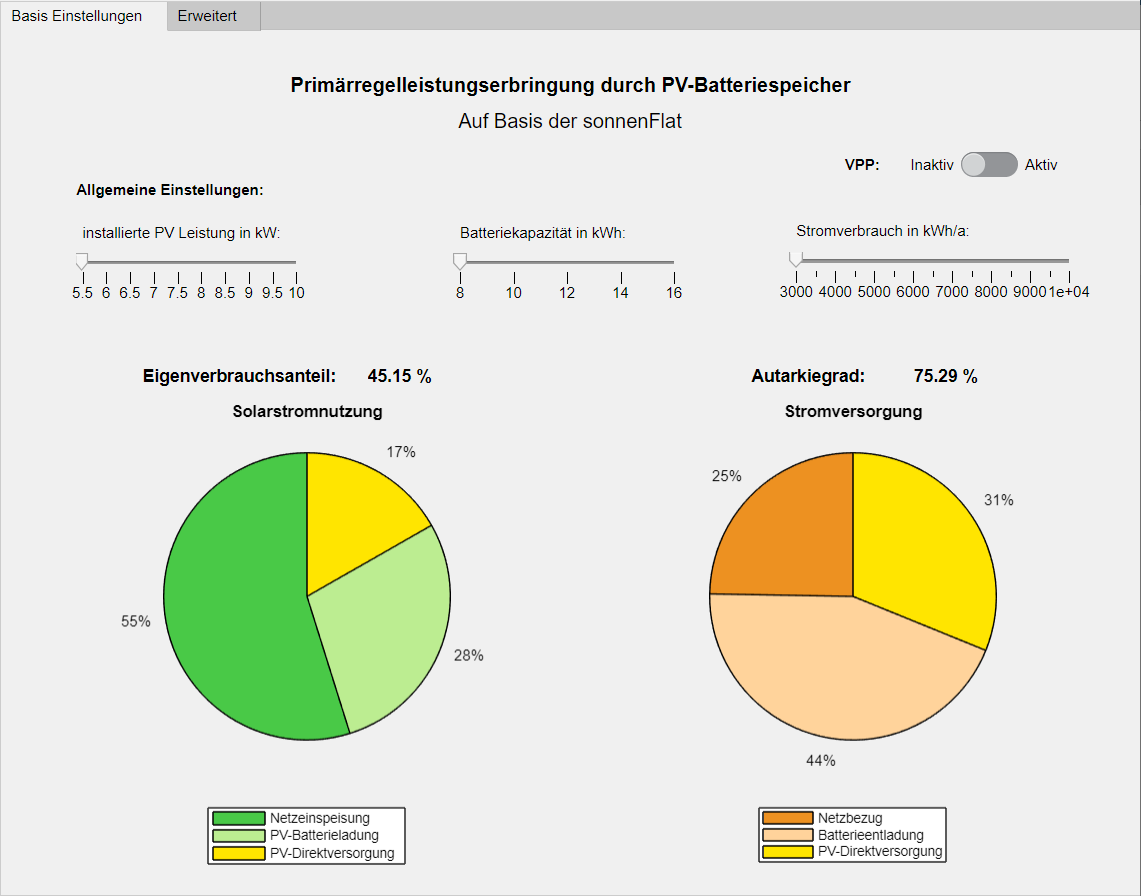
\includegraphics[width=\textwidth]{Bilder/N_ScreenshotApp1.png}
		\caption{Startseite der Anwendung}
		\label{fig:app1}
	\end{center}
\end{figure}

Der Schwerpunkt des zweiten Tabs liegt darin zu zeigen, ob sich das System finanziell für den Verbraucher rechnet. Zuerst wird der bisherige Stromtarif über die Regler für die Fixkosten und variablen Kosten eingestellt. Als nächstes kann die EEG-Vergütung, die man erhält, über ein Dropdown-Menü ausgewählt werden. Mithilfe der angegebenen Parameter entsteht Balkendiagramm, das die berechneten Kosten und Einnahmen mit und ohne virtuelles Kraftwerk übersichtlich gegenüberstellt. Die Kosten sind orange, bzw. negativ aufgetragen und die Einnahmen und der EEG-Bonus ist grün, bzw. positiv aufgetragen.  Darunter abgebildet sind außerdem die sich ergebenden Jahresbilanzen, sowie die Differenz dieser. Ist die Differenz positiv, d. h. kann mit dem virtuellen Kraftwerk Geld gespart oder mehr verdient werden, leuchtet das Lämpchen grün. In diesem Fall ist Einsatz des Speichers als Teil des virtuellen Kraftwerks zu empfehlen. Leuchtet das Lämpchen rot, ist davon abzuraten.
\begin{figure}[H]
	\begin{center}
		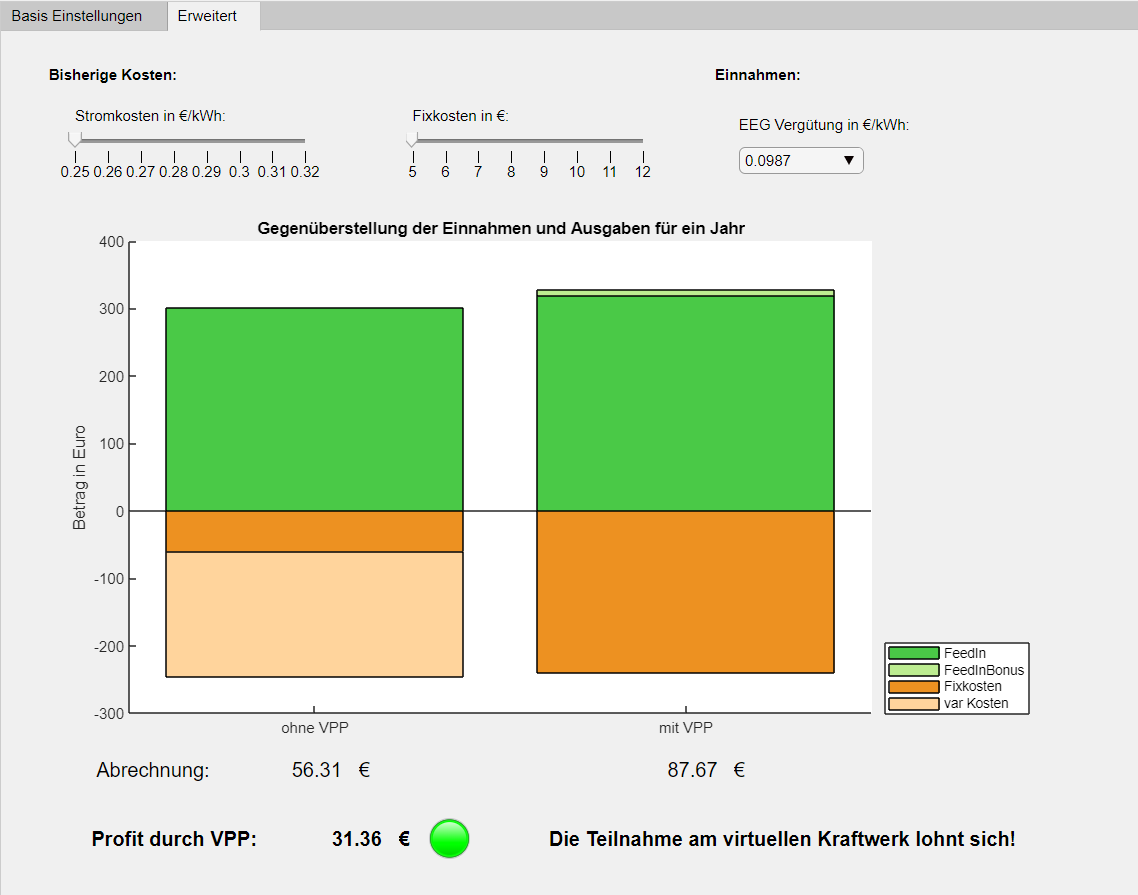
\includegraphics[width=\textwidth]{Bilder/N_ScreenshotApp2.png}
		\caption{Zweite Seite der Anwendung}
		\label{fig:app2}
	\end{center}
\end{figure}



\section{Ergebnisauswertung}

In den nachfolgenden Abschnitten werden die wichtigsten Ergebnisse der Simulation dargestellt und untersucht. Außerdem werden die relevanten Parameter einer Sensibilitätsanalyse unterzogen, um ihren Einfluss auf die Resultate zu quantifizieren.\medskip

\subsection{Ergebnisdarstellung}
Zunächst werden die entstandenen Extrempunkte betrachtet. Da das Ziel des Projekts primär die wirtschaftliche Beurteilung der Regelleistungserbringung durch PV-Batteriespeicher ist, werden die Fälle untersucht, in denen der direkte und indirekte finanzielle Verlust und Gewinn maximal sind. \\
Um diese Bedingungen zu definieren werden folgende Annahmen getroffen. Es ist davon auszugehen, dass bei aktivem VPP mehr Energie durch die PV-Anlage in das Netz eingespeist wird, da die Batterie aufgrund der geltenden SoC-Grenzen eine geringere Speicherkapazität bietet. Deswegen unterliegt der höchstmögliche Gewinn durch das VPP der Bedingung, dass die EEG Vergütung maximal ist. Umgekehrt ist der größte Verlust durch das VPP bei minimaler EEG Vergütung zu erwarten. Die Fixkosten und variablen Kosten, die nur die Bilanz ohne VPP beeinflussen, haben hingegen eine genau gegenteilige Wirkung. Je höher sie sind, desto günstiger ist es für den Wechsel zur SonnenFlat. \\
Die einzelnen Einnahme- und Kostenpunkte für die Extrempunkte sind in \ref{fig:Bilanz_minmax} aufgetragen. Das obere Balkendiagramm zeigt den günstigsten Fall. Konkret wird erreicht sich Maximum der Bilanzdifferenz bei 
\begin{itemize}
\itemsep-0.5em
	\item Einem Hausverbrauch von 10000{\kwh}
	\item Einer Kapazität der Batterie von 14{\kwh}
	\item Einer Größe der Photovoltaikanlage von 9.5{\kwp}
	\item Einer EEG-Vergütung für die Stromeinspeisung von 12.75{\ctkwh}
	\item Einem Grundpreis des Vergleichstromtarifs von 12{\Eurkwh}
	\item Einem Arbeitspreis des Vergleichstromtarifs von 32{\ctkwh}
\end{itemize}
erreicht. Die Einnahmen durch die Wirkung des VPPs belaufen sich auf maximal 849.02 Euro\\•
Die Zusammensetzung des Minimums der Bilanzdifferenz wird im unteren Diagramm abgebildet und befindet sich bei
\begin{itemize}
\itemsep-0.5em
	\item Einem Hausverbrauch von \SI{10000}{\kwh}
	\item Einer Kapazität der Batterie von \SI{16}{\kwh}
	\item Einer Größe der Photovoltaikanlage von \SI{7}{\kwp}
	\item Einer EEG-Vergütung für die Stromeinspeisung von \SI{9.87}{\ctkwh}
	\item Einem Grundpreis des Vergleichstromtarifs von \SI{5}{\Eurkwh}
	\item Einem Arbeitspreis des Vergleichstromtarifs von \SI{25}{\ctkwh}
\end{itemize}
Der maximale Verlust durch das VPP beträgt -321,60 Euro.
\begin{figure}[H]
	\begin{center}
		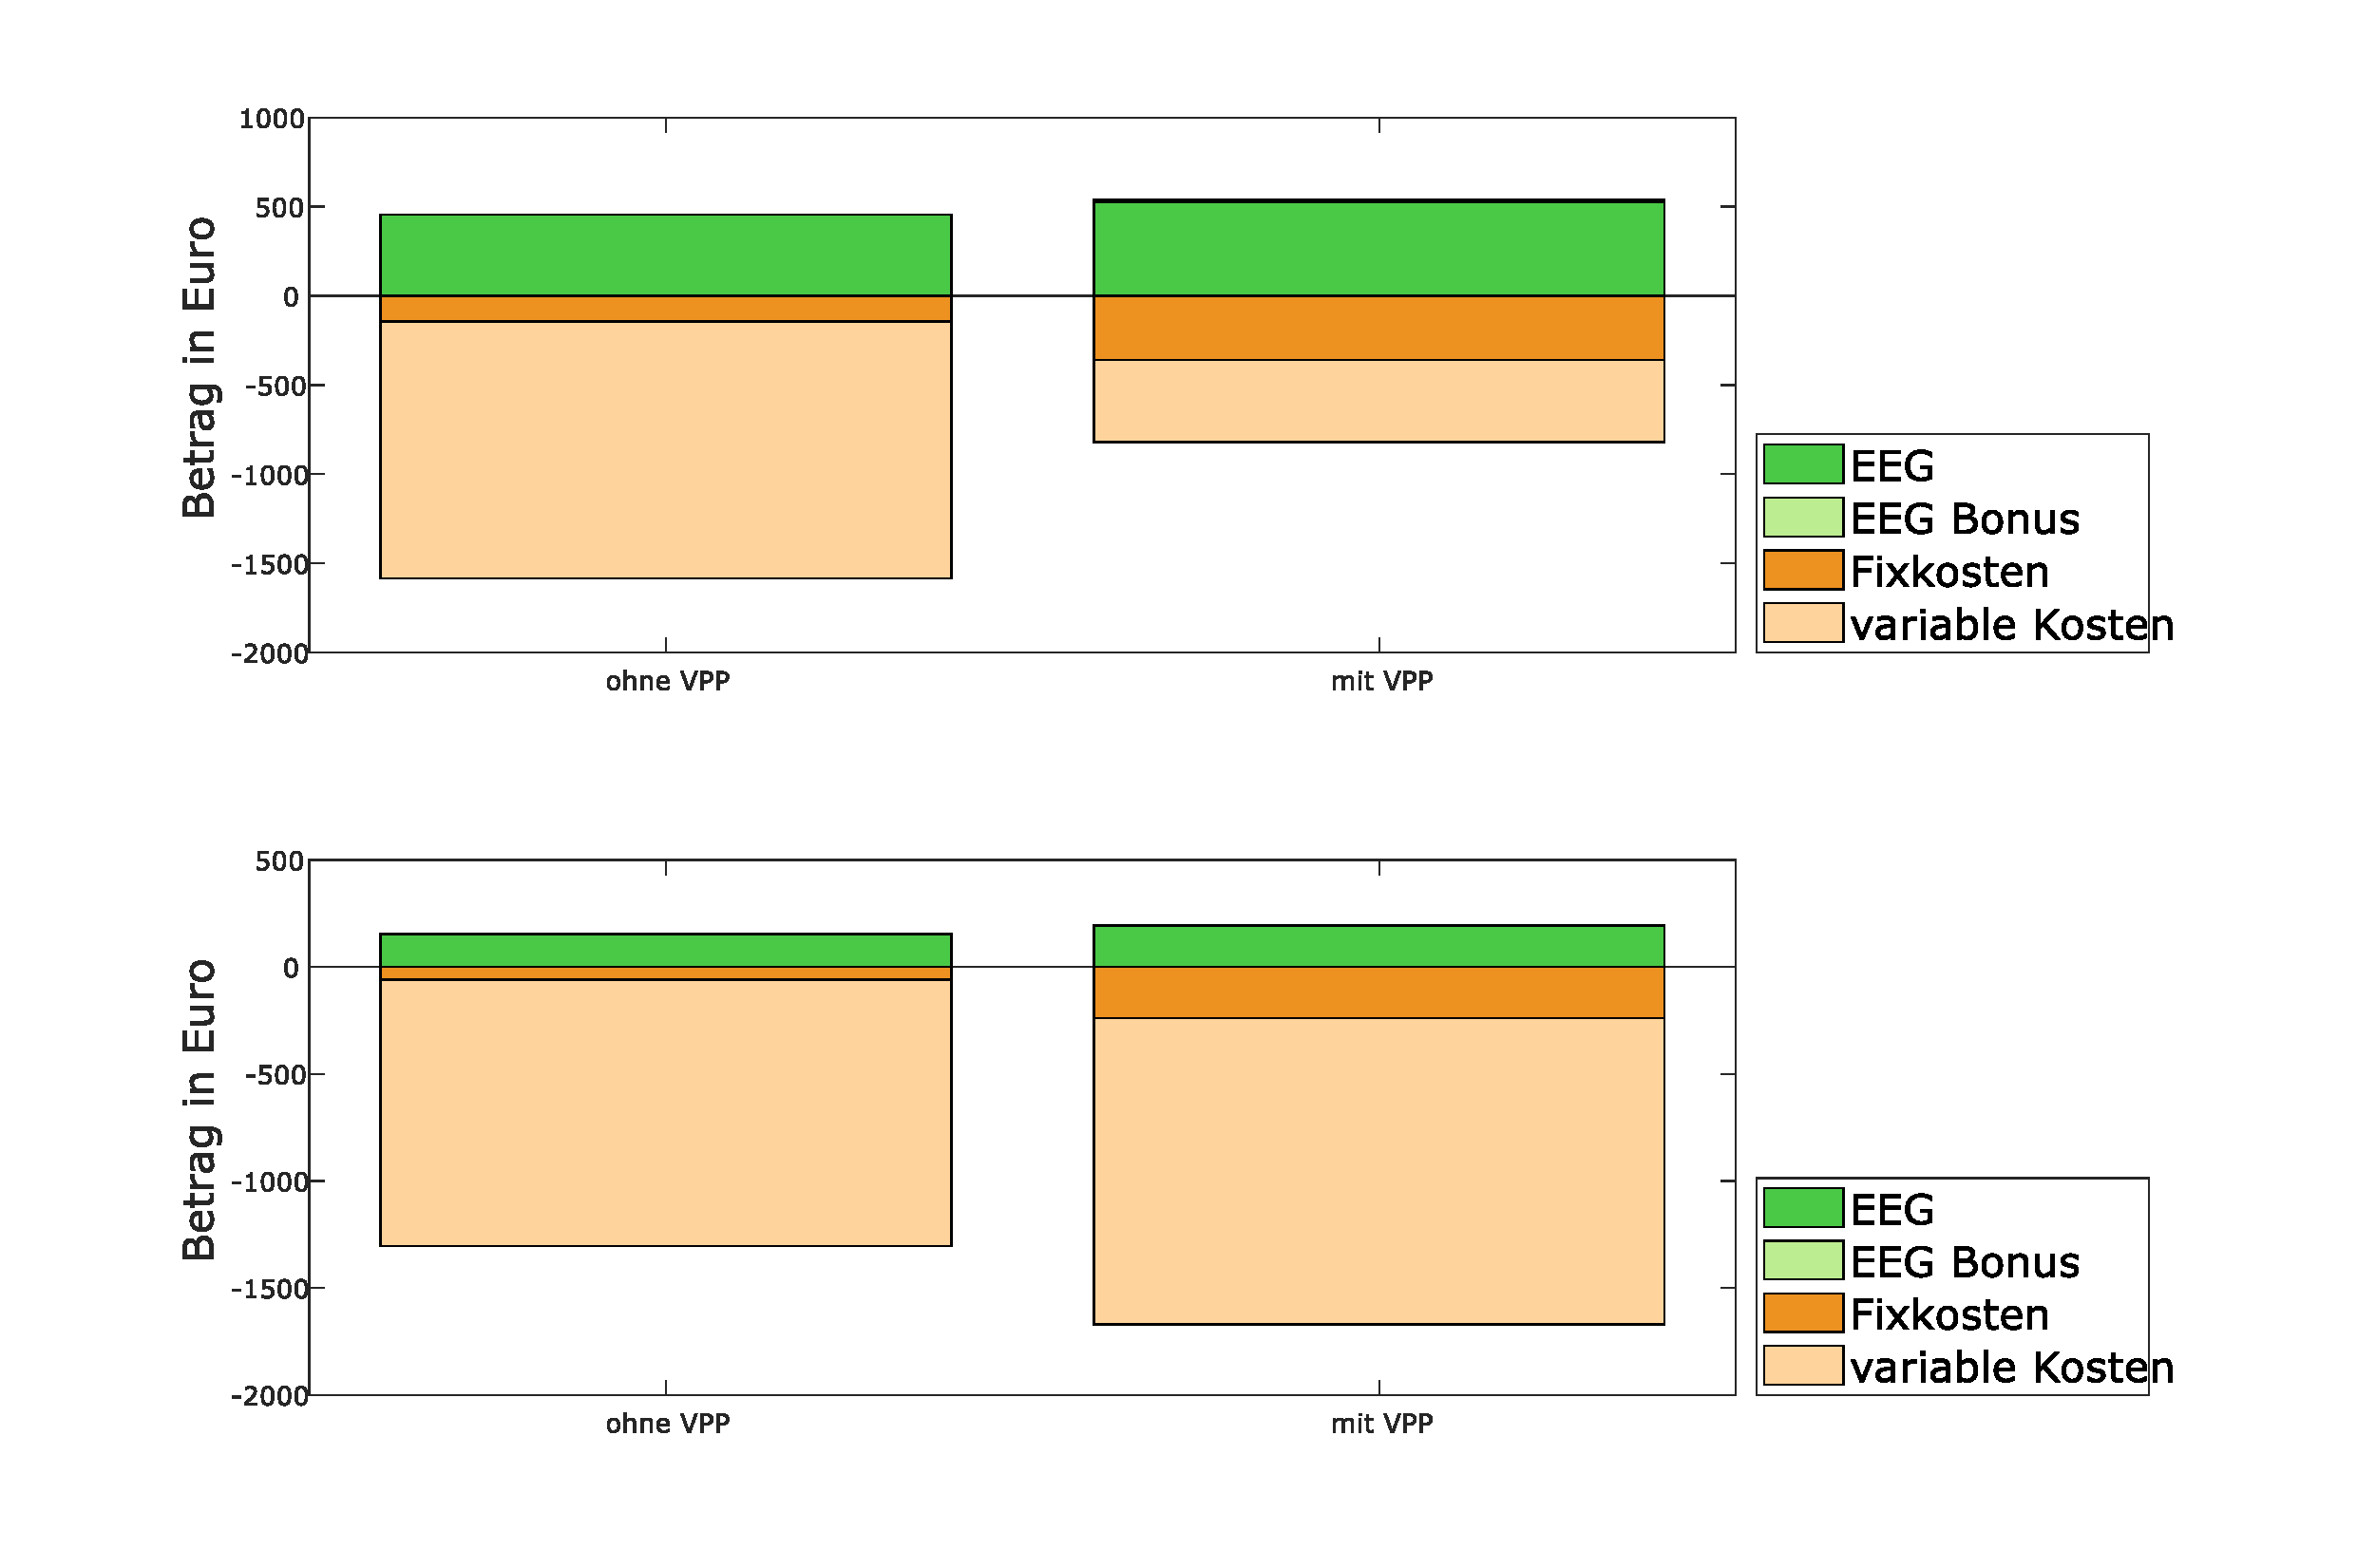
\includegraphics[width=\textwidth]{Bilder/Gegenueberstellung_Bilanz.pdf}
		\caption{Gegenüberstellung der Einnahmen und Kosten für den Verbraucher in zwei Fällen jeweils mit und ohne Regelleistungsbereitstellung für ein Jahr}
		\label{fig:Bilanz_minmax}
	\end{center}
\end{figure}

Ein Effekt, der langfristig zu finanziellem Verlust führen kann, ist die Zyklenbeanspruchung des Batteriesystems. Nach der Betrachtung des SoC ist eine höhere Auslastung der Batterie zu erwarten. Eine besonders hohe Zyklenzahl ist zu erwarten bei einer hohen installierten PV-Leistung, niedriger Batteriekapazität und hoher Last. \\
Betrachtet man nun die Simulationsergebnisse bestätigt sich dieser Verdacht.ist kaum ein Unterschied zu erkennen. Allerdings liegt die Anzahl der Zyklen mit VPP nicht übermäßig über der ohne, das Zyklenmaximum ohne VPP ist mit 296 sogar um 15 Ladegänge höher. Und auch das Minimum liegt mit 95 nur 17 niedriger als mit VPP. Nur mit dieser geringen Anzahl an Werten fällt es schwer eine aussagekräftige Wertung über den Einfluss von Regelleistungsbereitstellung abzugeben, wobei sie trotz alledem vermuten lassen, dass er nicht erheblich ist. Hinzu kommt, dass das SonnenBatterie System auch bei einer deutlich höheren Zyklenzahl noch garantiefähig ist, da diese erst nach 10.000 Zyklen bzw. 10 Jahren Gebrauch verfällt \cite{sonnenBat18}.
% Notizen: Hier noch Plot mit Zyklenzahl einbinden!

\subsection{Sensibilitätsanalyse}
% Einfluss der PV Leistung
% Einfluss der Batteriekapazität
% Einfluss der Last
% Einfluss der variablen Kosten
% Einfluss der EEG Umlage


														% Michi

\printbibliography[																				% Quellenverzeichnis ausgeben
	heading=bibintoc
]

\newpage

%\appendix

%%Appendix

\section{Anhang}


																		% Appendix

\end{document}
